\documentclass[conference]{IEEEtran}
\IEEEoverridecommandlockouts
% The preceding line is only needed to identify funding in the first footnote. If that is unneeded, please comment it out.
\usepackage{cite}
\usepackage{amsmath,amssymb,amsfonts}
\usepackage{algorithmic}
\usepackage{graphicx}
\usepackage{textcomp}
\usepackage{xcolor}
\usepackage{fontenc}
\usepackage[procnames]{listings}
\usepackage{lipsum,mwe,cuted}
\usepackage{float}%%%%提供浮动体的[H]选项，进而取消浮动
\usepackage{caption}%%提供captionof命令
\usepackage{booktabs} 
\usepackage{multirow}
\usepackage{tikz}
% \usepackage[table,xcdraw]{xcolor}
\usepackage{colortbl}
\usepackage{makecell}
\usepackage{pifont}
\usepackage{multirow}
\usepackage[hidelinks, colorlinks=true, linkcolor=black, urlcolor=blue, citecolor=black]{hyperref}

%https://www.overleaf.com/project/6448f4230b1ff94969d8d59f

\def\BibTeX{{\rm B\kern-.05em{\sc i\kern-.025em b}\kern-.08em
    T\kern-.1667em\lower.7ex\hbox{E}\kern-.125emX}}
\begin{document}

\title{Hierarchical Source-to-Post-Route QoR Prediction in High-Level Synthesis with GNNs\vspace{-0.5em}}

\author{\IEEEauthorblockN{Mingzhe Gao$^{1}$,
Jieru Zhao$^{1*}$, Zhe Lin$^{2*}$, Minyi Guo$^{1}$}
\IEEEauthorblockA{${}^{1}$Shanghai Jiao Tong University, ${}^2$Sun Yat-sen University\\
\{a823337391z,zhao-jieru\}@sjtu.edu.cn, linzh235@mail.sysu.edu.cn, guo-my@cs.sjtu.edu.cn}\vspace{-1cm}}


\maketitle
\begingroup\renewcommand\thefootnote{*}
\footnotetext{Jieru Zhao and Zhe Lin are the corresponding authors.}
\endgroup

\begin{abstract}
High-level synthesis (HLS) notably speeds up the hardware design process by avoiding RTL programming. However, the turnaround time of HLS increases significantly when post-route quality of results (QoR) are considered during optimization. To tackle this issue, we propose a hierarchical post-route QoR prediction approach for FPGA HLS, which features: (1) a modeling flow that directly estimates latency and post-route resource usage from C/C++ programs; (2) a graph construction method that effectively represents the control and data flow graph of source code and effects of HLS pragmas; and (3) a hierarchical GNN training and prediction method capable of capturing the impact of loop hierarchies. Experimental results show that our method presents a prediction error of less than 10\% for different types of QoR metrics, which gains tremendous improvement compared with the state-of-the-art GNN methods. By adopting our proposed methodology, the runtime for design space exploration in HLS is shortened to tens of minutes and the achieved ADRS is reduced to 6.91\% on average. Code and models are available at \url{https://github.com/sjtu-zhao-lab/hierarchical-gnn-for-hls}.
\end{abstract}

 \vspace{-0.13cm}   
\section{Introduction}
 \vspace{-0.1cm}  

High-level synthesis (HLS) enables users to create hardware designs at a high level of abstraction using programming languages like C/C++, and provides a series of pragmas, to tune hardware micro-architectures. Due to its superior productivity, HLS is becoming a popular solution for next-generation hardware development, especially for FPGAs. 
% Even though HLS is more efficient in producing register-transfer-level (RTL) designs compared with manual crafting, 
However, the turnaround time for HLS design is significantly increased when post-route quality of results (QoR), such as latency and resource utilization, are considered during optimization. To obtain an accurate assessment of post-route QoR metrics, a complete C-to-bitstream design flow should be invoked each time the HLS code is modified.  
% the hardware design to pass through the time-consuming RTL-based electronic design automation (EDA) flow, including logic synthesis, placement and routing. 
This runtime overhead undermines the benefits brought by HLS, especially when it comes to choosing the solution with optimal QoRs from an extremely large design space. 
% multiple design variants are generated by HLS and then assessed via the time-consuming RTL implementation flow to search for a solution with optimal QoR.
% i.e., the common practice for design space exploration. 
Therefore, it is essential to provide a fast and accurate QoR prediction framework at an early design stage like HLS to improve design efficiency.


%In the academia, early assessment of hardware performance and resource utilization has attracted a surge of research interest. These research works can be classified into two categories: analytical methods and learning-based methods. Analytical methods \cite{zhao2017comba,choi17} are developed by encompassing domain-specific knowledge from design experts, and they show exceptionally high accuracy in predicting performance, i.e., latency. However, there is a significant drawback of these analytical models. That is, the analytical models are specifically tailored for a pre-determined set of directives, largely restricting their applicability. In an effort to address the aforementioned issue, researchers have turned to machine learning techniques instead. In particular, the work \cite{7927161} introduces a method utilizing Gradient Boosting Machine, which starts from the source code, extracts features within the code, and predicts post-HLS performance and resource usage. Similarly, the work \cite{koeplinger2016automatic} adopts an artificial neural network approach to predict post-HLS resource usage. However, these approaches are unable to estimate post-route resource utilization, which leads to significant inaccuracies when they are applied to real applications that should be running onboard.

%In pursuit of more accurate QoR prediction for real applications, some studies~\cite{dai2018fast, makrani2019pyramid} seek to leverage HLS results in order to predict post-route QoR. The common practice of these works is to collect the results of the HLS design flow, extract features and employ machine learning techniques to estimate the post-route results. However, these works still have critical limitations: they require the invocation of the complete HLS flow, which incurs high timing cost when it comes to large-scale design space exploration. To carry out design space exploration more effectively, researchers further attempt to predict QoR with the source code. The studies in \cite{sohrabizadeh2022gnn, ferretti2022graph} make notable strides in this direction. These two works employ graph neural network (GNN) to explore the correlation between C/C++ programs and the QoR of their corresponding hardware implementation. Their innovative ideas of representing programs as graphs and applying GNN to model hardware performance and resource utilization lay the foundation for a promising solution to the prediction of post-route resource utilization.



Existing prediction methods can be classified into analytical and learning-based models. Analytical models are constructed based on domain expertise and achieve high accuracy in latency prediction \cite{zhao2017comba, choi17}. However, they are tailored for a specific subset of pragmas, resulting in limited scalability. Learning-based models adopt machine learning techniques \cite{7927161, dai2018fast, makrani2019pyramid} and graph neural networks (GNNs) \cite{sohrabizadeh2022gnn, ferretti2022graph,wu2022high} to predict latency and resource usage in HLS. We compare representative methods in Table \ref{tab:comp-related}. Zhong et al. \cite{7927161} extract features via source code profiling and use the gradient-boosted machine (GBM) to predict post-HLS metrics that can be obtained from HLS reports after synthesis. Then they conduct efficient DSE guided by their model. However, the labels in their dataset, i.e., post-HLS metrics, may deviate significantly from actual post-route QoR values. Hence, predicting post-HLS metrics may mislead the DSE process and get sub-optimal designs. Dai et al. \cite{dai2018fast} and Pyramid \cite{makrani2019pyramid} also utilize ML models while predicting post-route QoR metrics directly. However, their features come from HLS reports and necessitate the execution of the HLS flow, incurring a higher time cost. Recent advances introduce GNN models for QoR prediction due to their representation power of C/C++ programs. GNN-DSE \cite{sohrabizadeh2022gnn} and Ferretti et al. \cite{ferretti2022graph} represent source code as graphs and predict post-HLS metrics, which induce the same issue as \cite{7927161}. Wu et al. \cite{wu2022high} start from the HLS intermediate representation (IR) and predict post-route QoRs. They first predict resource types of operations and then incorporate the predicted resource types as node features to further estimate post-route resource usage. However, their input graphs are constructed on top of HLS IR, requiring running the HLS flow to generate related information. More importantly, the samples in their dataset exhibit relatively simple code structures, including randomly generated DFGs and loops without pragmas applied. The missing pragma modeling makes it less suitable for DSE tasks.    

% These two works employ graph neural network (GNN) to explore the correlation between C/C++ programs and the QoR of their corresponding hardware implementation. 

% However, this work does not involve the usage of directives and can only deliver QoR assessment results for the holistic designs, making it difficult to identify the bottleneck of a kernel, which still adversely impacts the efficiency and accuracy of design space exploration.

\begin{table}
\caption{Comparison between representative methods.}
\label{tab:comp-related}
\renewcommand\arraystretch{1}
\centering
\begin{tabular}{cccccc}
\hline
\makecell{} & \makecell{\textbf{Model}} & \makecell{\textbf{Input}} & \makecell{\textbf{Prediction} \\\textbf{Targets}} & \makecell{\textbf{Pragmas} \\ \textbf{Involved}} & \makecell{\textbf{HLS Exec.} \\\textbf{Free}} \\ \hline
\cite{7927161} & GBM & Source code & \makecell{Post-HLS} & \ding{51} & \ding{51} \\
\cite{dai2018fast} & XGB & \makecell{HLS reports} & \makecell{Post-Route} & \ding{55} & \ding{55} \\
\cite{sohrabizadeh2022gnn} & GNN & Source code & \makecell{Post-HLS} &  \ding{51} &  \ding{51}   \\
\cite{wu2022high}  & GNN & HLS IR & \makecell{Post-Route} & \ding{55} &  \ding{55} \\
Ours & GNN & Source code & \makecell{Post-Route} &  \ding{51} & \ding{51}   \\
\hline
\end{tabular}
\vspace{-0.5cm}
\end{table}







% \textcolor{blue}{Modify by MZ, compress paragraph}. 

% \textcolor{blue}{Origin: In pursuit ...}. To improve the efficacy of QoR prediction, some works~\cite{dai2018fast, makrani2019pyramid} try to predict post-route QoR from the HLS results. The common practice is to extract features from HLS and then learn to estimate QoR with machine learning techniques. However, they still require the invocation of the complete HLS flow, which is time-consuming for design space exploration. To address this, some works attempt to predict post-route QoR from source code directly. \textcolor{blue}{Origin: As one of ...}. As one of the state-of-the-art, \cite{wu2022high} presents an approach that predicts post-route resources and clock period from source code. It has a two-step flow: predicting HLS infomation for each operation, then embedding these as GNN node features, culminating in post-route resource and clock period prediction. However, lacking directives, it only assesses overall design QoR, limiting its efficiency in pinpointing design bottlenecks.

% Compared to the state-of-the-art work\cite{wu2022high}, our work provides a more advanced methodology in terms of post-route performance prediction for HLS. Our method takes into account the combination of multiple directives, as well as the effect of loop hierarchy in C/C++ programs. Specifically, we propose a hierarchical post-route QoR modeling method for FPGA HLS using up-to-date GNN techniques, which distinguishes itself from the prior arts with the following key features: 1) \textbf{accuracy}: our method demonstrates high accuracy for the estimation of post-route QoR metrics including performance and resource utilization, outperforming the state-of-the-art learning-based works; 2) \textbf{efficiency}: our method directly uses C/C++ source code as the input and gives a fast post-route estimation of latency and resource utilization without the need of invoking any traditional EDA design flow in the inference stage; and 3) \textbf{hierarchy reservation}: in contrast to the holistic QoR modeling works, our method presents the ability to infer QoR of different code hierarchies in loops and functions. We summarize our contribution as follows:

To summarize, few of the previous methods achieve accurate source-to-post-route QoR prediction. The problem is even more challenging if the code structure is complicated and multiple HLS pragmas are considered. Different from directly predicting QoR with the whole graph in previous methods, our insight is that we can reserve the structural information of loops/functions and predict post-route QoR metrics gradually from inner to outer hierarchies. This will reduce the estimation difficulty and potentially improve the prediction accuracy. 

To this end, we propose a \textit{hierarchical} prediction method using GNNs, which distinguishes itself from prior arts with the following key features: 1) \textbf{efficiency}: our method directly takes C/C++ source code as input and gives a fast post-route QoR estimation without invoking any EDA design flow, inlcuding HLS, during inference; 2) \textbf{pragma embedding:} we introduce an effective graph construction approach that jointly represents the control and data flow graph of source code and effects of HLS pragmas; 3) \textbf{hierarchical training and prediction}: our method is capable of capturing the structural information of code hierarchies and presents the ability to estimate QoR for different loop/function hierarchies; 4) \textbf{accuracy}: our method presents an average prediction error of $<$10\% for post-route QoR metrics, outperforming the state-of-the-art GNN methods. With efficient and accurate QoR estimation, the DSE time is shortened to tens of minutes and the achieved ADRS is reduced to 6.91\% on average.


% \begin{itemize}
% \item We design a modeling flow to estimate latency and post-route resource utilization for FPGA designs directly from C/C++ programs, without the invocation of the traditional EDA tools.
% \item We present a hierarchical GNN training method that preserves loop-based hierarchies of C/C++ programs and produces accurate post-route QoR estimation.
% \item We develop an innovative graph representation technique to jointly embed both the hardware micro-architectures and the HLS pragmas, which facilitates design space exploration for FPGA HLS.
% \end{itemize}

\vspace{-0.1cm} 
\section{PRELIMINARIES}
\vspace{-0.1cm} 

\subsection{Control and Data Flow Graph (CDFG)}
\vspace{-0.1cm} 


%\begin{figure} \centering
%	 \includegraphics[width=3.5in]{figure/CDFG.pdf} 
%	 \caption{Control and data flow graph}
% \vspace{-0.4cm}
%\label{fig_cdfg} 
%\end{figure}

%The Control Flow Graph (CFG) is an abstract representation of a process or program, serving as an abstract data structure used in compilers to represent the execution process of a program. It illustrates the potential flow direction of all basic blocks within a process in the form of a graph and can reflect the real-time execution process. Additionally, the Data Flow Graph (DFG) is another abstract representation, capturing the relationship of data dependencies.

%\textcolor{blue}{Modify by MZ, compress paragraph}.

%\textcolor{blue}{Origin: The Control ...}.
The Control Flow Graph (CFG) is a graphical representation of a program that describes the possible flows between basic blocks in the program. Likewise, the Data Flow Graph (DFG) is another graphical representation that depicts the dependencies between operations. By combining CFG and DFG, we obtain a Control and Data Flow Graph (CDFG). 
% Utilizing CDFG to represent programs offers several advantages: 1) CDFG can be acquired at the source code level, allowing for the earliest possible graph description of a program when predicting post-route performance in HLS; 2) CDFG can be generated with LLVM IR \cite{LLVM:CGO04}, enabling the extraction of numerous node-level information, which aids in predicting underlying hardware performance; 3) based on the loop structure in the source code, CDFG naturally reflects the hierarchy of loops, making it convenient to add optimization information for loops at different levels to the CDFG; 4) CDFG contains control flow and data flow information, assisting in distinguishing whether loops can be parallelized and determining whether resources can be shared.
%\textcolor{blue}{Origin: By combining ...}.
Using CDFG to represent programs offers several advantages: 1) CDFG can be generated with LLVM IR, allowing for the earliest possible graph description of a program; 2) CDFG naturally reflects hierarchies of loops, making it convenient to annotate loop-based information at different levels; 3) CDFG contains control and data flow information that can be used to distinguish whether loops can be parallelized and determine whether resources can be shared.

% it is possible to identify the potential of resource sharing from CDFG.


\vspace{-0.1cm} 
\subsection{Graph Neural Network}
\vspace{-0.1cm} 

%Graph Neural Networks (GNNs) are a class of neural networks designed to operate on graph-structured data. A graph is a data structure that represents objects as nodes and their dependencies as edges. GNNs utilize this representation to learn local and global relationships by aggregating information from neighbors and considering the overall graph structure. This makes them particularly useful for tasks such as node classification, link prediction, and graph-level prediction. The core idea of GNN models follows the "message passing" pattern: for each node $v \in V$ within a graph $G = (V, E)$, GNNs capture k-hop neighbor's information $h^k_{N_v}$ and subsequently learn an embedding $h^k_v$ after $k$ layers of processing. 

%\textcolor{blue}{Modify by MZ, compress paragraph}.

%\textcolor{blue}{Origin: Graph Neural Networks (GNNs)...}.
GNNs process graph-structured data, where objects are nodes and relationships are edges. GNNs learns node representation with a \emph{message passing} mechanism: each node \( v \) in the graph \( G \) collects the embedding \( h^k_{N_v} \) of its \( k \)-hop neighbor \({N_v}\) to update its embedding \( h^k_v \) after \( k \) graph convolution layers.

Since input C/C++ programs can be represented as graphs (i.e., CDFGs) naturally, GNNs become a powerful technique to capture features of each operation and recognize relationships between neighbor operations. Due to its representation power, we make full use of GNNs in a hierarchical way for the post-route QoR prediction.



%\section{Motivation and Challenges}
%\textcolor{red}{TODO: modify and add an example?}

%Considering the association between graphs and programs, we believe that GNN holds potential for forecasting specific performance metrics for programs. A considerable number of HLS directives are centered around loops, given that loop optimization plays a pivotal role in the process of HLS. When a loop is set with such a directive, it acquires global features unique to that directive. For instance, once a loop is appended with the \verb|#pragma HLS pipeline|, the initiation interval (II) becomes an important feature that is specific to this loop. However, obtaining this II value presents a challenge, as it cannot be directly derived from the program graph. Therefore, a more appropriate approach is to calculate its corresponding II using analytical model and use this feature as an overall characteristic of the loop for the network to process. Yet, in our program graph, a loop is merely a subgraph, complicating the addition of such unique features inherent to the loop.

%Hardware designs can be represented as graphs naturally. Therefore, we believe that GNNs hold great potential for forecasting hardware characteristics given C/C++ programs for HLS. However, it is non-trivial to incorporate HLS directives into commonly used graph representation. One reason is that the effective field of different HLS directives are different. For example, the loop-based directives, such as pipeline, operate on specific loop structures, which corresponds to a set nodes in the hardware graphs. In contrast, the function-based directives, such as dataflow, works on the complete function, i.e., a graph. Since the commonly used graph representation is flattened, these structural information, such as loops, has not been encapsulated naturally.

%From the above considerations, the idea of a GNN model based on loop hierarchy seems inevitable. However, with the plethora of pragmas in HLS, various combinations of pragmas can change the hierarchy of loops. The most typical examples are setting \verb|#pragma HLS pipeline| on the outer layer of a double loop, and setting \verb|#pragma HLS flatten| on the inner layer of a double loop. The former results in the complete unrolling of the inner loop of the double loop, whereas the latter merges nested loops into a single loop level. Ultimately, both will present as a single loop. Therefore, discerning loop hierarchy based on pragma, and setting up a reasonable GNN according to the corresponding hierarchy, are challenges we need to consider.

%The idea of constructing a GNN model that can encode loop hierarchies seems to be a promising solution to this problem. However, with the plethora of directives in HLS, the combinations of different directives may change the hierarchy of loops. Examples include setting \verb|#pragma HLS pipeline| on the outer-most level of a nested loop, and setting \verb|#pragma HLS flatten| on the inner-most level of a perfect nested loop. The former results in the complete unrolling of the inner loop of the nested loop, whereas the latter merges nested loops into a single loop level. Ultimately, both of the above two cases will change the loop structures in the source code with the corresponding directives inserted. Therefore, identifying loop hierarchy by considering the effects of directives, and building a GNN that can learn different hierarchies, are challenging.

%Moreover, it is also crucial to consider incorporating certain directives that aren't directly related to loops into the graph. An exemplar of such directives is \verb|#pragma HLS array_partition|. This directive plays a critical role in optimizing the memory access pattern, enabling simultaneous access to different portions of the array, which can significantly improve performance. Consequently, effective strategies are needed to integrate such directives into the graph, capturing their impact while maintaining the integrity of the loop hierarchy and the overall system model.

%Besides the above challenges, we also note that even some directives that are not relevant to loop structures can exert significant effect on loops. An example is the array directive \verb|#pragma HLS array_partition|. This directive splits the target array into multiple elements, which can increase the memory bandwidth for memory access of this array within loops. As a result, the loop-based graph representation method should also consider the effect of seemingly loop-independent directives on loops.

%In summary, we categorize the challenges of this task into the following key points:

%\begin{itemize}
%\item How to reasonably represent the global features inherent to loops in the graph.
%\item How to establish a reasonable hierarchy based on the plethora of directives, and set up a suitable GNN structure according to this hierarchical structure.
%\item How to represent a loop-independent directive within a graph, and effectively integrate the most pertinent features influenced by this directive into the graph
%\end{itemize}

%To address the aforementioned challenges, a model capable of learning to cluster various hierarchical nodes is essential. We put forth a pioneering methodology designed to facilitate the development of a more comprehensive model.

%In summary, we distill three key challenges for hierarchical QoR estimation targeting FPGA HLS:
%\begin{itemize}
%\item How to reasonably encode loop characteristics in the graph?
%\item How to jointly represent directives and hardware micro-architectures in the graph?
%\item How to consider the effect of seemingly loop-independent directives on loops?
%\item How to develop a GNN training mechanism that can embed loops with multiple hierarchies?
%\end{itemize}

%In the following Section~\ref{sec: method}, we illustrate the strategies we propose to overcome the above challenges.

%\begin{figure*}[t] \centering
%	 \includegraphics[width=7.5in]{figure/new architecture.pdf} 
%	 \caption{Method Architecture}
%\label{fig_sim} \end{figure*}



\begin{figure}
\centering
	 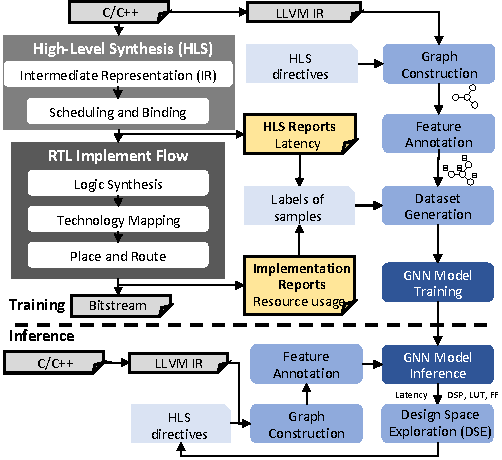
\includegraphics[width=0.45\textwidth]{figure/overview.pdf} 
	 \caption{Framework overview}
  \vspace{-0.6cm}
\label{fig_overview} \end{figure}

\vspace{-0.1cm} 
\section{Methodology}
\vspace{-0.1cm} 
\label{sec: method}

%Figure \ref{fig_overview} illustrates the overview of our proposed approach. There are two phases: GNN models are trained in the first phase (training) and accurate performance prediction and efficient design space exploration are conducted in the second phase (inference). During the training phase, the full-stack source-to-bitstream design flow is invoked to obtain the ground truth QoR considering various combinations of HLS directives. Specifically, the resource usage statistics are extracted from implementation reports after PAR and the latency statistics are acquired from HLS reports, since HLS resource estimations deviate greatly from the actual values after PAR while latency estimations are relatively accurate \cite{dai2018fast}. Our approach starts with the input source code (C/C++) which is transformed to LLVM IR. Then we select a rich set of combinations of HLS directives and construct a graph representation of the input code applied with different directive configurations (\textit{graph construction}). After that, several node and edge features are extracted and annotated to the graph for model training (\textit{feature annotation}). By bundling the annotated graphs and their corresponding ground truth labels under the same directive setting, our dataset can be generated (\textit{dataset generation}). In the final step, we train multiple GNN models for accurate post-route QoR prediction, while incorporating the inherent hierarchical nature of loops (\textit{GNN model training}). During the inference phase, accurate predictions of post-route performance are provided for a given input program, eliminating the need of invoking the entire source-to-bitstream design flow. Based on the fast feedback from the QoR prediction model, efficient design space exploration can then be conducted to search for the optimal configuration of directives that achieves the best performance. 

%\textcolor{blue}{Modify by MZ, compress paragraph}.

%\textcolor{blue}{Origin: Figure \ref{fig_overview} illustrates ...}.
Figure \ref{fig_overview} illustrates the overview of our proposed approach. 
% GNN models are trained in the first phase (training) and accurate performance prediction and efficient design space exploration are conducted in the second phase (inference). 
During the training phase, we deploy the complete C-to-bitstream design flow to obtain the ground-truth QoR considering various combinations of HLS pragmas. We extract resource statistics from implementation reports after place and route (PAR) and latency details from HLS reports. Our approach starts with the input source code (C/C++) which is transformed into LLVM IR. Then we construct a graph representation of the input code with different pragma configurations applied (\textit{graph construction}). After that, node and edge features are extracted and annotated in the graph (\textit{feature annotation}). By bundling the annotated graphs and their corresponding ground-truth labels under the same pragma configuration, our dataset can be generated (\textit{dataset generation}). In the final step, we train multiple GNN models for accurate post-route QoR prediction, while incorporating the inherent hierarchical nature of loops (\textit{GNN model training}). 
During the inference phase, accurate predictions of post-route performance are provided for a given input program, without invoking any HLS or RTL implementation flow. Based on the fast feedback from the prediction model, efficient DSE can then be conducted to search for the optimal configuration of pragmas that achieves the best performance. 

\vspace{-0.1cm}
\subsection{Graph Construction} \label{sec:graph contruction}
\vspace{-0.1cm} 

The input source code is first transformed to LLVM IR using the Clang front-end. Then we construct the corresponding graph representation by extending a CDFG generator, PrograML \cite{cummins2021a}, which captures both control and data flow. However, PrograML does not target FPGAs, and the generated program graphs need to be extended to consider the effects of HLS pragmas. Figure \ref{fig_graph} illustrates our graph construction process considering different kinds of pragmas.




\subsubsection{Constructing graph with loop pipelining} In a pipelined loop, the execution of consecutive iterations can be initiated after a specific interval, i.e., initiation interval (II). This is achieved by inserting registers into the logic during the synthesis process of HLS tools. The equivalent graph representation is not influenced or changed at the compilation stage. Therefore, the graphs constructed for pipelined loops remain the same as those of original loops without pipelining, as shown in Fig. \ref{fig_graph}(a). %\textcolor{blue}{Modify by MZ, delete some sentences}.% Each node represents operations and their edges denote data dependencies. To estimate the QoR performance of pipelined loops, the key point is to recognize the loop-carried dependencies and II, which further influence the estimation of latency and the degree of resource sharing. We consider these factors in \textit{feature annotation} by extracting critical features and annotating them to graph nodes.

\subsubsection{Constructing graph with loop unrolling} 
The loop unrolling pragma facilitates the concurrent execution of iterations and results in the creation of multiple replicas of hardware logic. In accordance with this principle, when constructing graphs for unrolled loops, the pertinent logic nodes in the unrolled region are replicated and appropriate edges are established to connect to original predecessors and successors. This procedure is illustrated in Fig. \ref{fig_graph}(b). By adding replicas of logic nodes explicitly, the resulting graph achieves a natural representation of \textit{loop unrolling} and significantly alleviates the complexity of prediction.


\subsubsection{Constructing graph with array partitioning} HLS tools provide the \textit{array partitioning} pragma to increase local memory bandwidth. Arrays are divided into smaller ones based on user-specified options. To reflect the impact of memory ports on performance estimation, we incorporate I/O port nodes to the original CDFG, as highlighted in orange in Fig. \ref{fig_graph}. When \textit{array partitioning} is applied, the corresponding memory port nodes are split into a certain number of nodes based on partitioning factors. These newly introduced memory port nodes are connected to load and store nodes that read from or write to corresponding memory locations. %\textcolor{blue}{Modify by MZ, delete some sentences}. 
The connections are determined by partitioning types as well as the memory access pattern of the code. Specifically, for a $k$-dimensional array, assuming its partition factors across the $k$ dimensions are $u_1, u_2, \cdots, u_k$, we add $\prod_{i=1}^{k} u_i$ memory port nodes in the graph. Simultaneously, we write LLVM passes to analyze the index values of each load and store operation to determine which memory ports should be connected to them.  If the array index is dynamic or unpredictable, the load/store nodes will connect to all memory ports. 


\begin{figure}
\vspace{-0.2cm}
        \centering
	 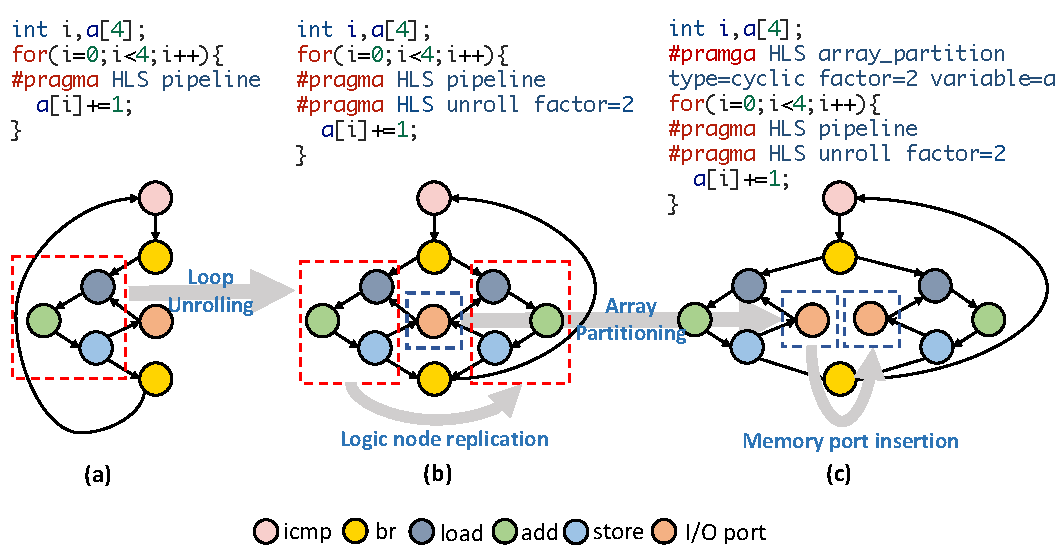
\includegraphics[width=3.5in]{figure/CDMGF.pdf} 
	 \caption{Procedure of graph construction.}
  \vspace{-0.5cm}
\label{fig_graph} \end{figure}

\vspace{-0.1cm}
\subsection{Feature Extraction and Annotation}
\label{ssec: feat}
\vspace{-0.1cm} 

Effective features need to be extracted from the code and annotated to the generated graph for model training. We categorize the features we have used into two categories: (1) node features and (2) loop-level features. 

\subsubsection{Node Features} Table \ref{tab-feature} summarizes our node features.
\textbf{Optype} denotes the operation type of each node, such as \verb|add|, \verb|mul|, \verb|div|, \verb|load|, \verb|store|. This is obtained by analyzing LLVM IR instructions. \textbf{\#invocation} denotes the number of times that an operation or a node is executed in a loop, which is associated with the loop tripcount and unroll factor. %\textcolor{blue}{Modify by MZ, delete some sentences}. % In our case, we traverse the LLVM IR to extract the tripcount which is divided by the unroll factor to compute \#invocation. 
\textbf{In and out degrees} represent the number of edges flowing into and out of the node, respectively, which can indirectly reflect the potential resource usage of multiplexers.
%Based on our generated graphs, the features of the nodes themselves can also provide significant support for the regression task. A key feature is the in-degree and out-degree of nodes, which can indirectly reflect the potential resource usage of multiplexers.
\textbf{Delay} and \textbf{\#cycle} represent the timing information of each operation/node, which helps latency prediction. We build a latency and delay library for each operation type based on profiling results from several micro-benchmarks.
For \textbf{LUT}, \textbf{DSP} and \textbf{FF}, we profile corresponding resource usage for arithmetic operations (e.g., \verb|add|, \verb|mul|, \verb|fadd|) using micro-benchmarks and build a library. For non-arithmetic operations (e.g., \verb|br|, \verb|icmp|, \verb|mux|), we simply set their resource-related features to zero. 


\begin{table}
\renewcommand\arraystretch{1.1}
\caption{Node features}
\vspace{-0.2cm}
\begin{center}
\setlength{\tabcolsep}{2mm}{
\begin{tabular}{cccc}
\hline
\textbf{Feature} & \textbf{Description} & \textbf{Values} \\
\hline
Optype    & operation type  & \verb|load|, \verb|etc.| \\
\#invocation     & the number of invocations & \verb|int| \\
In degree   & the number of incoming edge  & \verb|int| \\
Out degree    & the number of outcoming edge & \verb|int| \\
\#cycle  & the number of clock cycles  & \verb|int| \\
Delay  & the delay (ns) of each operation  & \verb|float| \\
LUT    & LUT usage of each operation & \verb|int| \\
DSP    & DSP usage of each operation & \verb|int| \\
FF   & FF usage of each operation & \verb|int| \\
\hline
\end{tabular}}
\label{tab-feature}
\end{center}
\vspace{-0.5cm}
\end{table}


\begin{figure*}
        \centering
	 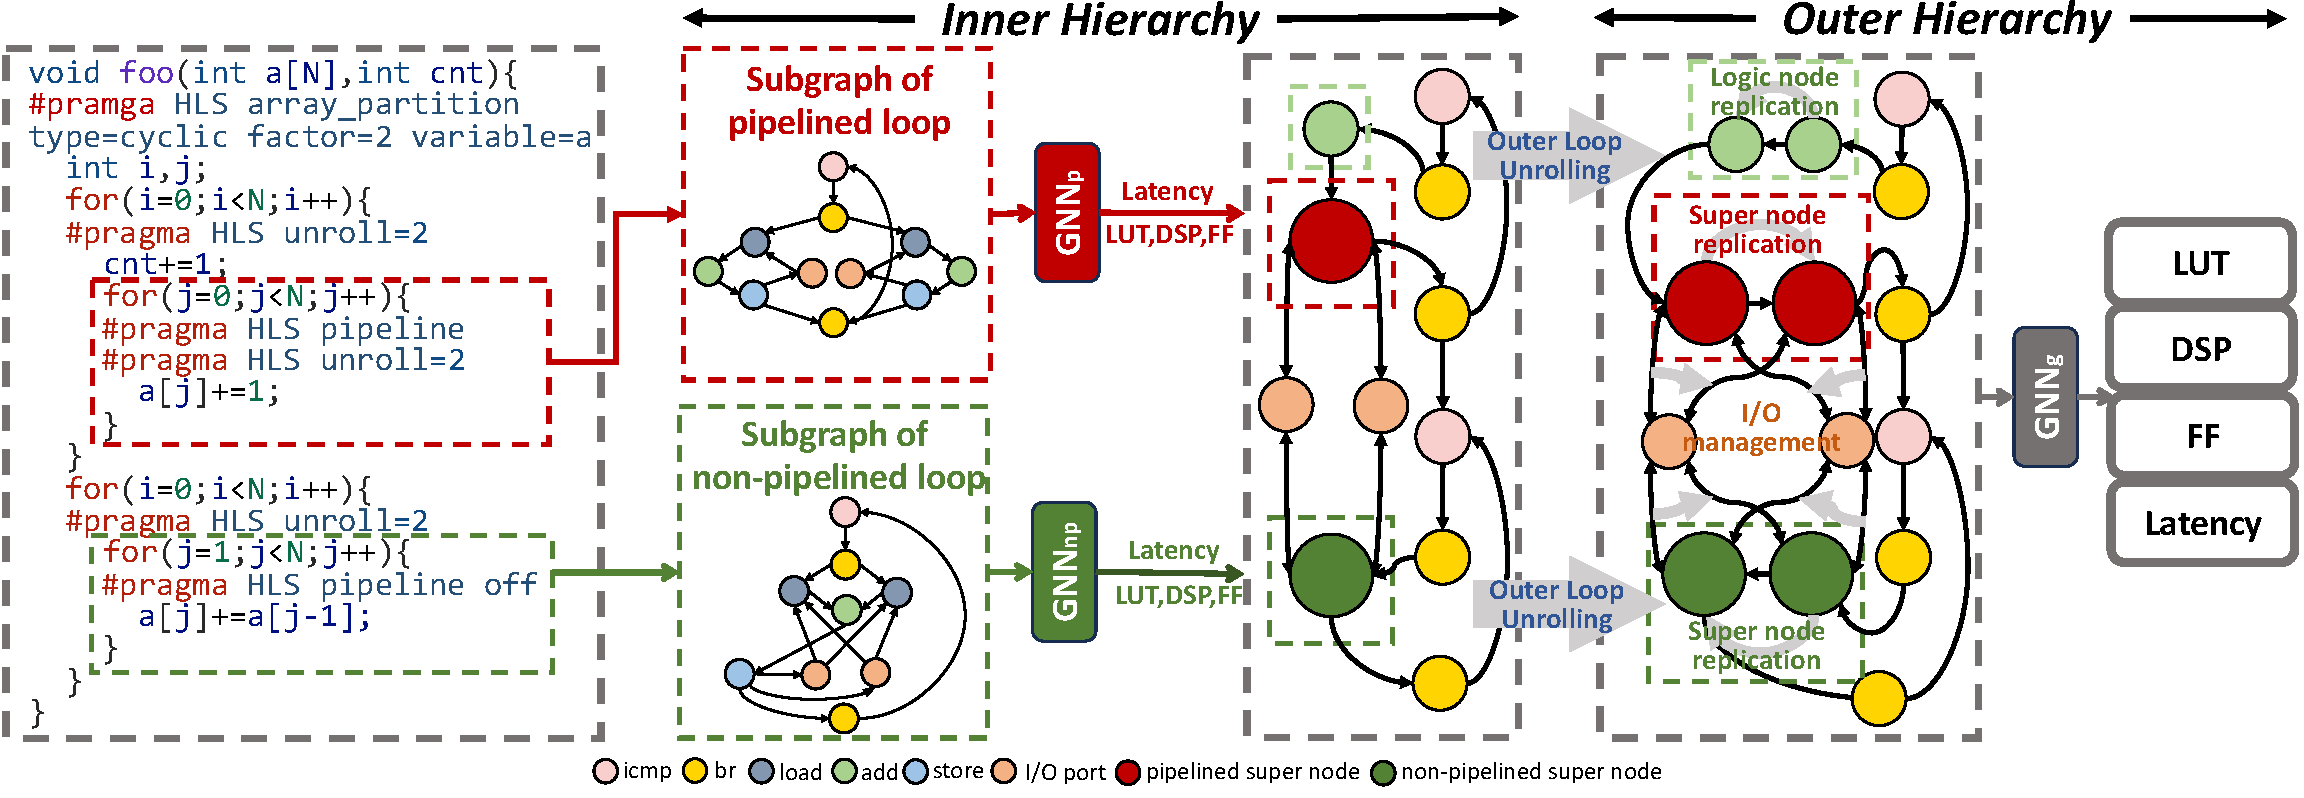
\includegraphics[width=0.95\linewidth]{figure/arch.pdf} 
	 \caption{The illustration of our hierarchical source-to-post-route QoR modeling approach.}
  \vspace{-0.4cm}
\label{fig_hierarchyGNN} \end{figure*}

%\textcolor{blue}{Modify by MZ, delete chain chance feature}.
%\textbf{Chain chance:} Operation chaining denotes that more than one operation can be scheduled in a single cycle if possible \cite{zhao2017comba}. This can influence our latency prediction. Suppose operation \verb|a| is followed by operation \verb|b|. Only when $\displaystyle \lceil \text{delay}_a/\text{clock period} \rceil = \lceil (\text{delay}_a+\text{delay}_b)/\text{clock period} \rceil$, is it possible for the two operations to be chained together. Therefore, we annotate all edges with a \verb|chain chance| feature to represent the possibility of operation chaining. If two operation nodes could potentially be completed within the same cycle, the \verb|chain chance| attribute of the edge connecting them is set to 1; otherwise, it is set to 0. 


\subsubsection{Loop-level features} Besides node features, we extract loop-level features so as to consider the effect of HLS pragmas on loops. As discussed in Section \ref{sec:graph contruction}, the graph of a pipelined loop remains the same as that of the loop without pipelining. Therefore, additional features should be considered to differentiate pipelining and non-pipelining. We use three features that determine the latency of a pipelined loop, namely, iteration latency (\textit{IL}), initiation interval (\textit{II}) and tripcount (\textit{TC}). Specifically, \textit{IL} can be approximated by GNNs and \textit{TC} can be obtained by analyzing the LLVM IR code, while II can be computed by the equation\cite{8695879}:
%However, \textit{II} is related to the loop-carried dependence and the availability of memory ports, which are hard to be captured by graph directly. Therefore, we compute a lower bound of \textit{II} \cite{zhao2017comba}:
\vspace{-0.1cm}
\begin{eqnarray*}
II_\textit{min} & = & \max(II^{rec}, II^{res}) \\
   & = & \max(\max\{\lceil \frac{\textit{Delay}_p}{\textit{Distance}_p} \rceil\}, \max\{\lceil \frac{\textit{Access}_m}{\textit{Ports}_m} \rceil\})
\end{eqnarray*}
where Delay$_p$ represents the latency between a pair of dependent instructions from different iterations, Distance$_p$ refers to the difference between the corresponding iteration numbers, Ports$_m$ is the number of ports and Access$_m$ is the number of accesses to array $m$. %\textcolor{blue}{Modify by MZ, delete some sentences}.
%It is important to note that the lower bound of \textit{II} may differ from the actual synthesized \textit{II}. However, it can still provide informative hints for the GNN regression. Besides, if \textit{II} is user-specified by setting the \textit{loop pipelining} directive, we directly use this input \textit{II} value as the feature. 




\vspace{-0.1cm} 
\subsection{The Hierarchical Modeling Approach}
\label{ssec: model}
\vspace{-0.1cm} 

After constructing and annotating graphs, the complete C-to-bitstream flow is invoked to obtain the ground truth QoR considering various HLS pragmas. Then the annotated graphs and their corresponding QoR labels form our dataset for model training. The detailed setup is discussed in Section \ref{sec:experiment setup}. 

We propose a hierarchical source-to-post-route QoR modeling methodology, as depicted in Fig. \ref{fig_hierarchyGNN}. To capture and incorporate the inherent hierarchical nature of loops, we train multiple GNN models to estimate QoR results at different loop hierarchies and gradually predict the overall latency and resource usage of the application. Our method can be generalized to applications with multiple nested loops. Take the code in Fig. \ref{fig_hierarchyGNN} as an example, the top function \textit{foo} has two nested loops, each with two loop levels, i.e., loop hierarchies. In the first nested loop, its sub-loop at the inner hierarchy (\textit{j-level}) is pipelined and partially unrolled, and its sub-loop at the outer hierarchy (\textit{i-level}) is partially unrolled with factor two. This configuration creates a circuit with two replicas of the inner loop pipeline within the outer loop. The QoR of inner replicas greatly impacts the overall QoR of the nested loop. Thus, our strategy models the QoR of sub-loops at the inner hierarchy using a local GNN, merges inner sub-loops to \textit{super nodes}, and integrates super nodes with operations at the outer hierarchy 
to model overall QoR with a global GNN. 


% Following the natural loop hierarchies, the difficulty of QoR prediction is reduced since we divide the problem into several smaller issues. 
% The accuracy of QoR prediction can also be improved significantly, compared with a single GNN used in previous works \cite{wu2022high}, because fine-grained features at different loop hierarchies can be detected and captured. To be more specific, we divide loop hierarchies into two levels: \textbf{inner and outer hierarchies}. 

This hierarchical approach simplifies post-route QoR prediction by dividing the problem into smaller ones. It also improves estimation accuracy by capturing fine-grained features at different hierarchies, compared to previous GNN methods that directly predict performance with the whole graph. To be more specific, we divide loop hierarchies into two levels: \textbf{inner and outer hierarchies}. 

\subsubsection{Inner Hierarchy}
In our method, a loop at the \textbf{inner hierarchy} denotes the loop that only contains computing logic without sub-loops. There are four types of loops that belong to the inner hierarchy: \ding{172} a single-level loop; \ding{173} a nested loop with \textit{loop pipelining} applied to the outermost level (in this case, all the inner sub-loops will be fully unrolled); \ding{174} a perfect nested loop with \textit{loop flattening} and \textit{loop pipelining} applied to the innermost level (in this case, all the loop levels will be flattened to form a deeper pipeline which is equivalent to a single-level pipelined loop); and \ding{175} a nested loop with all the inner sub-loops fully unrolled. For example, in Fig. \ref{fig_hierarchyGNN}, the two j-level loops in red and green boxes are loops at the inner hierarchy, corresponding to category \ding{173} and \ding{172}, respectively.
At the inner hierarchy, related loops are first extracted and subgraphs are constructed for model training, as illustrated in Fig. \ref{fig_hierarchyGNN}. Then we train two different GNN models, namely $\textbf{GNN}_p$ and $\textbf{GNN}_{np}$, to predict QoR for pipelined and non-pipeline loops, respectively. This is because execution models of pipelined and non-pipelined loops are different and training GNN models separately can improve accuracy based on our experiments. After predicting the QoR of loops at the inner hierarchy, the nodes in a subgraph 
% that form a loop at the inner hierarchy 
are merged into a super node, which represents this loop at the inner hierarchy when modeling the outer hierarchy. 
% The super nodes are connected to other logic nodes from the outer hierarchy to form the complete graph representation of the top function \textit{foo}. Since the outer loop is unrolled, corresponding logic nodes and super nodes are replicated according to the unrolling factor, following the same strategy as discussed in Section \ref{sec:graph contruction}.

\subsubsection{Outer Hierarchy} We define all the remaining logic and loop levels as components at the \textbf{outer hierarchy}. Note that loops can contain more than two loop levels. After the first stage, we condense each loop at the inner hierarchy into a super node. These super nodes are connected to the nodes from the outer hierarchy to form the complete graph representation of the top function \textit{foo}. If the outer loop is unrolled, corresponding logic and super nodes are replicated following strategies discussed in Section \ref{sec:graph contruction}. In the entire program graph, we 
% replace the inner-loop structures with super nodes and 
annotate super nodes with predicted QoR as features. Each super node holds a complete set of node features as shown in Table~\ref{tab-feature}, where features such as \verb|LUT|, \verb|DSP|, \verb|FF|, \verb|latency| are derived from the previous prediction phase. The calculation method used for other features remains consistent with those of standard logic nodes. This program graph, containing super nodes and logic nodes of the outer hierarchy, becomes the input graph of our global GNN model named $\textbf{GNN}_g$. The global GNN model is trained to predict the final QoR of the whole application. This approach not only assists us in predicting the overall performance of real applications more accurately but also helps in discerning serial and parallel relationships between super nodes, i.e., loops.

\begin{figure*}
    \centering
	 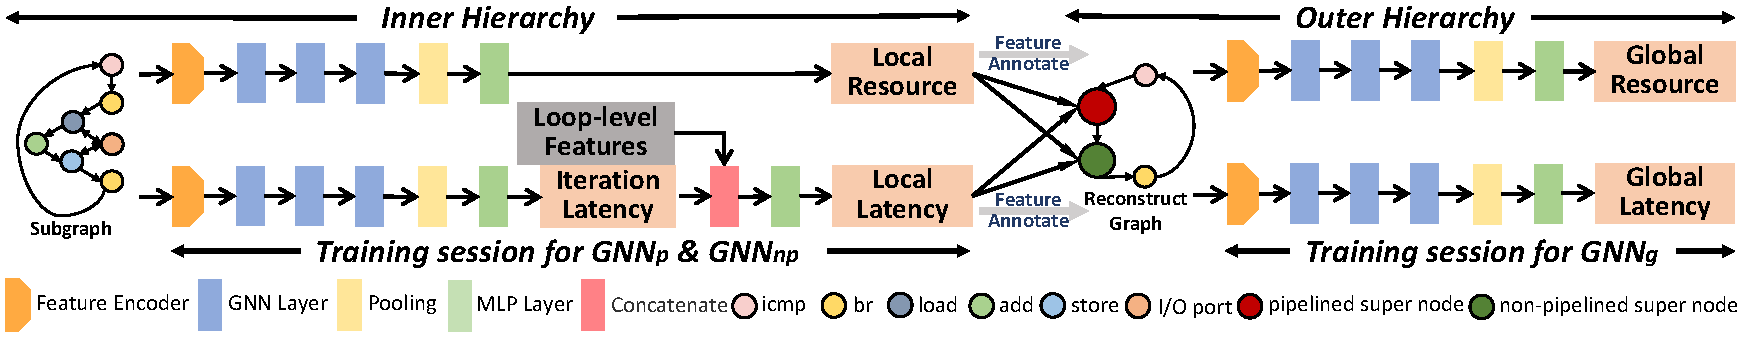
\includegraphics[width=0.95\linewidth]{figure/GNNarch.pdf} 
	 \caption{GNN architectures and the corresponding hierarchical training process.}
\label{fig_GNNarch} 
\vspace{-0.3cm}
\end{figure*}

\vspace{-0.15cm} 
\subsection{GNN Architectures and Training Process} 
\label{gnnarch}
\vspace{-0.1cm} 

We develop three GNN models for the prediction of each QoR metric, namely $\textbf{GNN}_p$, $\textbf{GNN}_{np}$, and $\textbf{GNN}_g$. 
Due to different execution models on hardware, $\textbf{GNN}_p$ and $\textbf{GNN}_{np}$ are deployed for pipelined and non-pipelined loops at the inner hierarchy, respectively. $\textbf{GNN}_g$ is used for prediction at the outer hierarchy. Figure \ref{fig_GNNarch} illustrates the model architectures and our hierarchical training process. 
%后面的内容需要根据图4来说明和重新组织：1. 怎么训练的，hierarchical training，freeze前面权重，再训练后面的；2. model architecture的特点。
The training process of the three GNN models is carried out in a hierarchical way. We initially collect the loops at the inner hierarchy, categorize them into pipelined loops and non-pipelined loops, and extract information from the two kinds of loops to generate corresponding datasets. Then $\textbf{GNN}_p$ and $\textbf{GNN}_{np}$ are trained accordingly. Once the training process is completed, the weights of both $\textbf{GNN}_p$ and $\textbf{GNN}_{np}$ are frozen. The output of these two GNNs is then used as features of super nodes, which are combined with features of other operations at the outer hierarchy to generate the dataset for training $\textbf{GNN}_g$. 


% \textcolor{blue}{Rather than training local model (i.e., $\textbf{GNN}_p$ and $\textbf{GNN}_{np}$) and global model (i.e., $\textbf{GNN}_g$) in isolation, our hierarchical training strategy enables the global model to discern the nuanced errors emerging from the local model, allowing the global model to make adjustments to these local errors and ensures that the error of the overall model does not become excessively large after several times of GNN inference.}

Our GNN models have similar architectures, as depicted in Fig. \ref{fig_GNNarch}. Each model can be decomposed into 1) feature encoder, 2) propagation layer, 3) pooling layer, and 4) MLP layer.  The \textit{feature encoder} converts the attributes of nodes into initial feature vectors. We use one-hot encoding for the attribute \verb|optype|, while numerical attributes are directly incorporated into the feature vector. \textit{Propagation layers} implement the message-passing mechanism of GNNs. We adopt the propagation layers from typical GNN models: GCN~\cite{kipf2017semi}, GAT~\cite{velickovic2018graph}, GraphSAGE~\cite{hamilton2017inductive}, TransformerConv~\cite{shi2020masked}, and PNA~\cite{Corso2020PrincipalNA}.
%\textcolor{blue}{Modify by MZ, compress paragraph}
After passing through three propagation layers, node embeddings are obtained. 
Then we use a \textit{pooling layer} to generate graph-level embeddings from node embeddings. We use two types of pooling: sum pooling \(h_{sum}\) and max pooling \(h_{max}\). The embeddings from these two pooling mechanisms are concatenated to form the graph-level representation.
%, as given by:
%$$
%h = \left( \sum u_i \right) \oplus \left( \max \{u_i\} \right)
%$$
%where $u_i$ denotes the feature vector of the $i^{th}$ node.
Finally, \textit{MLP layers} are used to project the graph-level embeddings into QoR prediction. For resource usage, we directly obtain the estimates after feeding the embeddings of the GNN into an MLP layer. For latency prediction, we handle the inner hierarchy ($\textbf{GNN}_p$ and $\textbf{GNN}_{np}$) and the outer hierarchy ($\textbf{GNN}_{g}$) separately. Regarding the inner hierarchy, first, $\textbf{GNN}_p$ and $\textbf{GNN}_{np}$ utilize an MLP layer to predict iteration latency. Second, another MLP layer takes the predicted iteration latency and loop-level features (elaborated in Section~\ref{ssec: feat}) as input and infers the latency of the loops at the inner hierarchy. Regarding the outer hierarchy, we directly predict the overall latency with an MLP.




%\subsubsection{Node \& Edge Encoder} Subsequently, We iterate over the attributes of each nodes and edges, encode these attributes, and then concatenate the resulting encodings to produce the initial embeddings. For the node feature vector, we use one-hot encoding for the \verb|optype| feature, while other features are embedded as their corresponding numerical values into the feature vector, resulting in a 43-dimensional node feature vector. For the edge feature vector, we employ one-hot encoding for both the \verb|chain chance| features, ultimately yielding a 2-dimensional feature vector.

%\textcolor{blue}{Modify by MZ, delete edge feature}



%\subsubsection{Propagation layer} Propagation layers implement the message-passing mechanism of GNNs. In the experiments, we evaluate six GNN models with different types of propagation layers, which are: 1) GCN\cite{kipf2017semi}, a fundamental GNN model that captures local neighborhood information by applying convolution operations on graphs; 2) GAT\cite{velickovic2018graph}, which utilizes attention mechanisms to weigh neighboring node features adaptively, enabling the model to focus on the most relevant information; 3) GraphSAGE\cite{hamilton2017inductive}, a GNN model that generates embeddings by sampling and aggregating features from a node's local neighborhood, allowing for efficient inductive learning on large graphs; 4) TransformerConv\cite{shi2020masked}, a GNN layer that utilizes the Transformer architecture, emphasizing attention mechanisms to better capture global information and node relationships; 5) PNA\cite{Corso2020PrincipalNA}, a GNN layer focusing on a wider range of aggregation functions, enabling a more comprehensive node feature learning and representation.

%\textcolor{blue}{Modify by MZ, compress paragraph}




%As for latency, different strategies are used for different GNNs. %For $\textbf{GNN}_p$, we note that the II calculated by the analytic model is inaccurate, and directly computing pipelined latency with the estimated II leads to inaccuracy. Therefore, $\textbf{GNN}_p$ is responsible for the prediction of iteration latency, then we concatenate the predicted iteration latency with the global loop features, and finally use an MLP to predict the sub-loop latency. For $\textbf{GNN}_{np}$, we can easily compute the sub-loop latency by multiplying the trip count by the iteration latency. Therefore, the MLP layer is not needed for $\textbf{GNN}_{np}$. In $\textbf{GNN}_g$, due to the absence of a loop structure, we can directly calculate the overall latency.
% For $\textbf{GNN}_p$ and $\textbf{GNN}_{np}$, we note that some of the global loop features, such as II calculated by the analytic model is inaccurate, and directly computing pipelined latency with the estimated II leads to inaccuracy. Therefore, we concatenate the predicted iteration latency with the global loop features and use an MLP to predict the sub-loop latency. For $\textbf{GNN}_g$, we directly predcit the overall latency with an MLP.

%\textcolor{blue}{Modify by MZ, delete training details}
%Extra training details: The training process for $\textbf{GNN}_p$, $\textbf{GNN}_{np}$, and $\textbf{GNN}_g$ is carried out separately. We initially extract information from the inner-most loops and categorize them into pipelined loops and non-pipelined loops. The former is fed into $\textbf{GNN}_p$ for training, while the latter is input to $\textbf{GNN}_{np}$. Once the training is completed, the weights of both $\textbf{GNN}_p$ and $\textbf{GNN}_{np}$ are frozen. The output of these two GNNs is then used as features of super nodes for training $\textbf{GNN}_g$. This training scheme ensures that the error of the overall model does not become excessively large after several times of GNN inference.


\vspace{-0.15cm}
\section{Experiments}
\vspace{-0.12cm}

\subsection{Experimental setup} \label{sec:experiment setup}
\vspace{-0.12cm} 

Our feature construction and model development flow is fully automated and implemented using Python and C++. We utilize 16 applications from the Polybench, MachSuite and CHStone benchmark suite. Specifically, 12 applications are used for GNN model training and testing, and 4 applications are used for the DSE experiment. The datasets to develop $\textbf{GNN}_p$ and $\textbf{GNN}_{np}$ are constructed based on sub-loops extracted from the application source code, while the dataset for $\textbf{GNN}_g$ is constructed based on the complete applications. Our experiments are conducted on the AMD Ultrascale+ MPSoC ZCU102. %We use Vitis-HLS 2022.1 and Vivado 2022.1 to generate latency and post-route resource utilization, respectively, which are then used as ground-truth labels for model training and evaluation. Together with the directive set (loop pipeline, loop unroll, loop flatten and array partition), we generate up to 3102 valid design points for $\textbf{GNN}_p$, 2300 valid design points for $\textbf{GNN}_{np}$ and 6178 valid design points for $\textbf{GNN}_g$. These datasets are randomly divided into a portion of 80\% for training, 10\% for validation, and 10\% for testing. Each model is trained five times over 250 epochs, with the model exhibiting the lowest validation loss being selected. We use the mean absolute percentage error (MAPE) to quantify the prediction quality.
%\textcolor{blue}{Modify by MZ, compress paragraph, origin: We use ...}
We utilize Vitis-HLS 2022.1 and Vivado 2022.1 to collect ground-truth latency and resource usage as training labels. By applying various pragma combinations, we produce 3102, 2300 and 6178 valid designs to build \(\textbf{GNN}_p\), \(\textbf{GNN}_{np}\), and \(\textbf{GNN}_g\), respectively. 80\% of the dataset is used for training, 10\% of the dataset is used for validation, and the remaining 10\% of the dataset is used for testing. We use the mean absolute percentage error (MAPE) to quantify the prediction quality. Each model is trained with over 250 epochs.

\begin{table}
\caption{MAPE of post-route QoR with different GNNs.}
\label{tab:predication}
\centering
\setlength{\tabcolsep}{1mm}{
\begin{tabular}{c|cccccc}
\hline
\textbf{GNN type} &    & \textbf{Latency}  & \begin{tabular}[c]{@{}c@{}}\textbf{Iteration}\\ \textbf{Latency }\end{tabular}& \textbf{DSP}  & \textbf{LUT}  & \textbf{FF}  \\ \hline
\multirow{3}{*}{GCN}  
& $\textbf{GNN}_p$      & 5.23\%     & 7.21\% & 4.94\% & 6.63\%  & 7.83\%  \\
& $\textbf{GNN}_{np}$       & 8.41\% & 8.41\% & 9.35\% & 5.88\%  & 8.39\% \\
& \cellcolor{lightgray} $\textbf{GNN}_g$      & \cellcolor{lightgray}9.85\% &\cellcolor{lightgray} N/A & \cellcolor{lightgray}7.45\% & \cellcolor{lightgray}11.27\% & \cellcolor{lightgray}11.24\% \\
\hline
\multirow{3}{*}{GAT}  
& $\textbf{GNN}_p$       & 4.91\% & 7.89\%  & 4.67\%  & 9.12\% & 9.20\%  \\
& $\textbf{GNN}_{np}$       & 9.42\% & 9.42\%  & 10.64\%  & 6.99\% & 9.32\%  \\
&\cellcolor{lightgray} $\textbf{GNN}_g$      & \cellcolor{lightgray} 10.88\% & \cellcolor{lightgray} N/A & \cellcolor{lightgray} 8.18\%  &  \cellcolor{lightgray}12.34\%  & \cellcolor{lightgray}11.57\% \\
\hline
\multirow{3}{*}{GraphSage}
& $\textbf{GNN}_p$ & 5.24\% & 5.52\%   & 5.88\%  & 8.12\% & 8.66\%   \\
& $\textbf{GNN}_{np}$ & 7.47\% & 7.47\% & 9.83\% & 6.25\% & 7.22\%   \\
& \cellcolor{lightgray}$\textbf{GNN}_g$ &\cellcolor{lightgray} 8.55\% &\cellcolor{lightgray} N/A & \cellcolor{lightgray}\textbf{6.94\%} &\cellcolor{lightgray} 9.86\% & \cellcolor{lightgray} \textbf{9.99\%} \\
\hline
\multirow{3}{*}{Transformer}
& $\textbf{GNN}_p$ & 4.92\% & 5.95\% & 4.05\% & 6.70\% & 7.12\% \\
& $\textbf{GNN}_{np}$ & 8.77\% & 8.77\%  & 12.02\%  & 5.83\% & 8.65\% \\
& \cellcolor{lightgray}$\textbf{GNN}_g$ & \cellcolor{lightgray}\textbf{8.54\%} & \cellcolor{lightgray}N/A & \cellcolor{lightgray} 6.97\% &  \cellcolor{lightgray}11.33\% & \cellcolor{lightgray} 10.31\%  \\
\hline
\multirow{3}{*}{PNA}
& $\textbf{GNN}_p$       & 6.74\% & 7.43\% & 4.11\%  & 8.92\%  & 9.93\%  \\ 
& $\textbf{GNN}_{np}$       & 9.99\% & 9.99\% & 10.55\% & 7.89\% & 10.26\%  \\ 
& \cellcolor{lightgray}$\textbf{GNN}_g$       & \cellcolor{lightgray}9.29\% &\cellcolor{lightgray} N/A &\cellcolor{lightgray} 7.84\% & \cellcolor{lightgray}\textbf{9.65\%} &\cellcolor{lightgray} 10.55\%  \\
\hline
\end{tabular}}
\vspace{-0.4cm}
\end{table}

\vspace{-0.1cm} 
\subsection{Evaluation of QoR prediction accuracy}
\vspace{-0.1cm} 

As introduced in Section \ref{gnnarch}, we adopt five different GNN models and compare their QoR prediction accuracy, as shown in Table \ref{tab:predication}. For loop-level models ($\textbf{GNN}_p$ and $\textbf{GNN}_{np}$), we present prediction errors for both latency and iteration latency. For application-level models ($\textbf{GNN}_g$), the latency prediction error of complete designs is reported. Among all the GNN models for application-level prediction, Transformer, GraphSage, and PNA achieve the lowest estimation errors in latency (8.54\%), DSP usage (6.94\%) and FF usage (9.99\%), and LUT usage (9.65\%), respectively. Our hierarchical method leads to high prediction accuracy of post-route QoR for pipelined loops ($\textbf{GNN}_p$), non-pipelined loops ($\textbf{GNN}_{np}$) and the complete applications ($\textbf{GNN}_g$), showing prediction errors of less than 10\% for latency and all types of resources. Since our method directly takes the C/C++ source code as input to predict the post-route QoR of FPGA designs without invoking any EDA tool flow, the prediction accuracy is highly desirable. 


%\begin{table}
%\caption{Prediction error (MAPE) of post-route QoR with different GNNs}
%\centering
%\setlength{\tabcolsep}{1mm}{
%\begin{tabular}{ccccccc}
%\toprule
%                     & \textbf{GNN type}   & \textbf{Latency}  & \begin{tabular}[c]{@{}c@{}}\textbf{Iteration}\\ \textbf{Latency }\end{tabular}& \textbf{DSP}  & \textbf{LUT}  & \textbf{FF}  \\ \hline
%\multirow{6}{*}{$\textbf{GNN}_p$}  
%& GCN       & 5.23\%     & 7.21\% & 4.94\% & \textbf{6.63\%}  & 7.83\%  \\
%& GAT       & \textbf{4.91\%} & 7.89\%  & 4.67\%  & 9.12\% & 9.20\%  \\
%& GraphSage & 5.24\% & \textbf{5.52\%}   & 5.88\%  & 8.12\% & 8.66\%   \\
%& Transformer & 4.92\% & 5.95\% & \textbf{4.05\%} & 6.70\% & \textbf{7.12\%} \\
%& PNA       & 6.74\% & 7.43\% & 4.11\%  & 8.92\%  & 9.93\%  \\ 
%\hline
%\multirow{6}{*}{$\textbf{GNN}_{np}$} 
%& GCN       & 8.41\% & 8.41\% & \textbf{9.35\%} & 5.88\%  & 8.39\% \\
%& GAT       & 9.42\% & 9.42\%  & 10.64\%  & 6.99\% & 9.32\%  \\
%& GraphSage & \textbf{7.47\%} & \textbf{7.47\%} & 9.83\% & 6.25\% & \textbf{7.22\%}   \\
%& Transformer & 8.77\% & 8.77\%  & 12.02\%  & \textbf{5.83\%} & 8.65\% \\
%& PNA       & 9.99\% & 9.99\% & 10.55\% & 7.89\% & 10.26\%  \\ 
%\hline
%\multirow{6}{*}{$\textbf{GNN}_g$} 
%& GCN       & 9.85\% & N/A & 7.45\% & 11.27\% & 11.24\% \\
%& GAT       & 10.88\% & N/A & 8.18\%  & 12.34\%  & 11.57\% \\
%& GraphSage & 8.55\% & N/A & \textbf{6.94\%} & 9.86\% & \textbf{9.99\%} \\
%& Transformer & \textbf{8.54\%} & N/A & 6.97\% & 11.33\% & 10.31\%  \\
%& PNA       & 9.29\% & N/A & 7.84\% & \textbf{9.65\%} & 10.55\%  \\
%\bottomrule
%\end{tabular}}
%\vspace{-2mm}
%\end{table}
\vspace{-0.1cm} 
\subsection{Comparison with the state-of-the-art}
\vspace{-0.1cm} 

We compare our method with the approach \cite{wu2022high} which also predicts post-route QoR using GNNs. Different from\cite{wu2022high}, we additionally consider various pragma combinations, increasing the complexity of code structures. For a fair comparison, we evaluate both methods on the dataset from \cite{wu2022high} which does not consider HLS pragmas and our dataset with pragmas, as shown in Table \ref{tab:comparison}. Without pragmas, our method and \cite{wu2022high} achieve close prediction accuracy, while on the dataset with pragmas applied, our method demonstrates superior improvement in all QoR metrics. We attribute this notable improvement to the following two reasons: 1) \textit{joint representation of code and pragmas during graph construction}: we deploy a graph construction method that represents the CDFG of source code while taking into account the impact of pragmas. This approach effectively embeds the pragma information into the graph representation. 2) \textit{reservation of loop hierarchies}: with our hierarchical training approach, messages can propagate more effectively between different levels of loop hierarchies, allowing GNNs to better understand the cascading effects of changes in the design's inner hierarchy on the outer hierarchy.


\begin{table}
\caption{Comparison of prediction error (MAPE).}
\vspace{-0.2cm}
\label{tab:comparison}
\begin{center}
\begin{tabular}{cccccc}
\hline
\textbf{Method} & \textbf{Configuration} & \textbf{Latency} & \textbf{DSP} & \textbf{LUT} & \textbf{FF} \\ \hline
\cite{wu2022high}  & w/o pragma & N/A & 8.26\% & 5.10\% & 7.58\%  \\
Ours & w/o pragma & 5.54\% & 6.71\% & 6.78\% & 7.91\% \\
\hline
\cite{wu2022high}  & w/ pragma & 35.81\% & 57.31\% & 27.14\% & 29.03\% \\
Ours & w/ pragma & 8.54\% & 6.94\% & 9.65\% & 9.99\% \\     
\hline
\end{tabular}
\label{tab1}
\end{center}
\vspace{-0.5cm}
\end{table}

%We tested our approach against theirs on both a randomly generated DFG dataset\cite{wu2022high} without pragmas and a application dataset with pragmas. The results clearly demonstrate the superiority of our method when handling datasets with pragmas. Table III shows the QoR prediction error for both our method and \cite{wu2022high}. From this, we can observe that without adding pragma, the results from our method are quite similar to theirs, suggesting that the feature addition in our approach is both logical and effective. On the other hand, when pragma is added, our method demonstrates superior performance over \cite{wu2022high} in all evaluation metrics, effectively showcasing the superiority of the hierarchical model in handling pragma. We attribute this notable improvement to the following two observations. (1) \textit{Combination of designs and directives}: by subtly integrating both hardware micro-architectures and HLS directives into the graph samples, we enables the GNNs to capture their effects and interactions during model development. (2) \textit{Advanced information propagation mechanism}: with our hierarchical training approach, messages can propagate more effectively between different levels of the hierarchies, allowing the GNNs to better understand the cascading effects of changes in one hierarchy of the design on the outer hierarchies.

%\textcolor{blue}{Modify by MZ, compress paragraph, origin: We tested our approach ...}

\vspace{-0.2cm} 
\subsection{Evaluation of Design Space Exploration}
\vspace{-0.1cm} 

%To demonstrate the effectiveness of our prediction method in helping with design optimization, we additionally perform DSE on the target applications, the objective of which is to find optimal directives configurations that produce the the Pareto frontier of hardware designs with the best design metrics including performance and different types of resources on FPGA. We implement a straightforward DSE algorithm based on the following two principles. (1) For each loop in the kernel, we start from the innermost loop and move to the outer loop, and in the meanwhile, we apply three types of directives: \verb|#pragma HLS pipeline|, \verb|#pragma HLS flatten|, and \verb|#pragma HLS unroll|. The unroll factor is selected from \{1, 2, 4, 8, 16\}. (2) To apply \verb|#pragma HLS array_partition| on the IO and internal buffers, we make the array partitioning factor consistent with the unroll factors of the loop that uses the buffer. This enables maximum possible parallel memory access for the loops. Under these two principles, we leverage our trained QoR estimator with GraphSage to predict the post-route QoR of the design points in the test set, following which the approximate Pareto frontier is derived. 

%\textcolor{blue}{Modify by MZ, compress paragraph, origin: To demon}
To demonstrate the effectiveness of our hierarchical QoR prediction method, we perform DSE on four new applications (\verb|bicg|, \verb|symm|,  \verb|mvt| and \verb|syrk|) that are unseen by our model during training. The design space of each application is constructed by varying pragma configurations. Specifically, we apply HLS pragmas like \textit{loop pipelining}, \textit{loop flattening} and \textit{loop unrolling} iteratively from inner to outer loops, with unroll factors from \{1, 2, 4, 8, 16\}. As for \textit{array partitioning}, we set partitioning factors consistent with unroll factors. 

The objective of DSE is to find the optimal pragma configurations producing the best QoR metrics, which form the Pareto frontier. To quantify the optimality, the average distance from reference set (ADRS) can be computed:
\vspace{-0.1cm}
\begin{equation*}
\text{ADRS}(\Gamma, \Omega) = \frac{1}{|\Gamma|} \sum_{\gamma \in \Gamma} \min_{\omega \in \Omega} f(\gamma, \omega),
\end{equation*}

where $\Gamma$ is the exact Pareto-optimal set, $\Omega$ is the approximate Pareto-optimal set, and $f(\cdot)$ computes the distance between two design points. A lower ADRS means that the approximate Pareto set is closer to the exact one. 
%Compared to Vivado, which requires several days of DSE for each kernel, our model demonstrates significant performance improvements during the DSE process. 

To get the exact Pareto-optimal set, we exhaustively evaluate the actual post-route QoRs for each design configuration by invoking the complete C-to-bitstream flow. Vitis HLS and Vivado are utilized to generate the accurate results. We then select the models with the highest prediction accuracy in Table \ref{tab:predication} to provide quick QoR estimation for DSE. For comparison, two other GNN models from \cite{wu2022high} and GNN-DSE~\cite{sohrabizadeh2022gnn} are tested similarly on the same design space. GNN-DSE~\cite{sohrabizadeh2022gnn} is one of the state-of-the-art works in HLS DSE. It uses a GNN-based post-HLS QoR prediction model to address the DSE problem.
The comparison of DSE results is shown in Table \ref{tab:dse}. 
The design space contains up to 2796 design configurations. The DSE time shows the timing costs required to finish the exploration with the QoR feedback from Vivado and from our model, respectively. By utilizing our method, efficient QoR feedback is provided, only necessitating constructing an IR graph from the C-level code followed by several rounds of GNN inference. This effectively bypasses the tedious steps of synthesis and implementation and shortens the DSE time from tens of days to tens of minutes. 


Compared to the work~\cite{wu2022high} and GNN-DSE~\cite{sohrabizadeh2022gnn}, which achieve average ADRS values of 13.94\% and 10.96\%  respectively, our method reaches an average ADRS of 6.91\%, demonstrating our superior ability to enable a high-quality DSE. The result fully verifies that the high accuracy of our predictive model can lead to a more precise approximation to the exact Pareto frontier. Regarding the runtime, both GNN-DSE and our method complete the exploration within minutes, while the method\cite{wu2022high} requires one to two days to complete due to the invocation of HLS tools. In summary, by incorporating our hierarchical prediction method, fast and accurate performance feedback can be provided to boost the efficiency of DSE.

%\textcolor{red}{version 1: } \textcolor{blue}{Experimental results indicate that our hierarchical QoR GNN model is a high-quality and light-weight alternative to the Vivado design flow regarding DSE. Our experiment explores up to 2796 design configurations for each kernel, achieving a maximum runtime speedup of 4235$\times$ compared to Vivado which demands several days of DSE for each kernel. Moreover, compared to the work~\cite{wu2022high} and GNN-DSE~\cite{sohrabizadeh2022gnn}, where their methods achieve average ADRS values of 13.94\% and 10.96\% respectively, our approach attains an average ADRS of 6.91\%. This indicates that our method offers a more accurate approximation of the exact Pareto frontier than the proposed works. In all, this case study shows promise for effectively boosting the efficiency of DSE by incorporating our hierarchical GNN-based QoR model. }

% \textcolor{red}{version 2: } \textcolor{blue}{Experimental results indicate that our hierarchical QoR GNN model is a high-quality and light-weight alternative to the Vivado design flow regarding DSE. In our experiment, we explore 2796, 1792, 2116, and 1972 design configurations for bicg, syrk, mvt, and symm respectively. Compared to Vivado, which requires 26 days, 44 days, 25 days, and 40 days to complete the DSE for each kernel, our model can accomplish the DSE in just tens of minutes. Moreover, compared to the work~\cite{wu2022high} and GNN-DSE~\cite{sohrabizadeh2022gnn}, where their methods achieve average ADRS values of 13.94\% and 10.96\% respectively, our approach attains an average ADRS of 6.91\%. This indicates that our method offers a more accurate approximation of the exact Pareto frontier than the proposed works. In all, this case study shows promise for effectively boosting the efficiency of DSE by incorporating our hierarchical GNN-based QoR model. }



% Experimental results indicate that our hierarchical QoR GNN model is a high-quality and light-weight alternative to the Vivado design flow regarding DSE, which can provide a close approximation of the exact Pareto frontier, while presenting three orders of magnitude improvement in runtime. Moreover, our method presents more accurate approximation of the exact Pareto frontier compared with the work~\cite{wu2022high} and GNN-DSE~\cite{sohrabizadeh2022gnn}. In all, this case study shows promise for effectively boosting the efficiency of DSE by incorporating our hierarchical GNN-based QoR model. 


%\begin{table}
%\caption{DSE performance on unseen applications.}
%\label{tab:dse}
%\centering
%\setlength{\tabcolsep}{0.5mm}{
%\begin{tabular}{c|c|cc|ccc}
%\hline
%\textbf{Kernel} & \begin{tabular}[c]{@{}c@{}}\textbf{\#Design}\\ \textbf{Config}\end{tabular} & \begin{tabular}[c]{@{}c@{}}\textbf{DSE} \\ \textbf{Time} \end{tabular} & \begin{tabular}[c]{@{}c@{}}\textbf{DSE Time}\\ \textbf{with Vivado} \end{tabular} & \begin{tabular}[c]{@{}c@{}}\textbf{\cite{wu2022high}}\\ \textbf{ADRS(\%)}\end{tabular} &  \begin{tabular}[c]{@{}c@{}}\textbf{\cite{sohrabizadeh2022gnn}}\\ \textbf{ADRS(\%)}\end{tabular} & \begin{tabular}[c]{@{}c@{}}\textbf{Ours}\\ \textbf{ADRS(\%)}\end{tabular} }  \\
%\hline
%bicg  & 2796 & 12m & 26d$\times$ &  12.13  & 9.14 & 6.39   \\
%symm  & 1972 & 15m & 44d$\times$& 13.15  & 11.50 & 5.45     \\
%mvt  & 2116 & 14m & 25d$\times$& 16.01 & 12.17 & 9.31  \\
%syrk & 1972 & 15m & 40d$\times$&  14.45& 11.03 & 6.49 \\
%\hline
%\end{tabular}}
%\label{dseruntime}
%\vspace{-5mm}
%\end{table}


% Please add the following required packages to your document preamble:
% \usepackage{multirow}
\begin{table}
\caption{DSE results on unseen applications.}
\vspace{-0.2cm}
\label{tab:dse}
\centering
\begin{tabular}{c|c|cc|ccc}
\hline
\multirow{2}{*}{\textbf{Kernels}} & \multirow{2}{*}{\textbf{\makecell{\#Design \\ Config}}} & \multicolumn{2}{c|}{\textbf{DSE time}} & \multicolumn{3}{c}{\textbf{ADRS(\%)}} \\ \cline{3-7} 
                         &                                  & \textbf{Vivado}        & \textbf{Ours}        & \textbf{\cite{wu2022high}}      & \textbf{\cite{sohrabizadeh2022gnn}}      & \textbf{Ours}      \\ \hline
bicg                     &    2796                          &  26 days           &  12 min        & 12.13       &  9.14      &  6.39      \\
symm                     &    1972                          &  44 days           &  15 min        & 13.15       &  11.50      &  5.45      \\
mvt                      &    2116                          &  25 days           &  14 min       &  16.01      &    12.17    &   9.31     \\
syrk                     &    1972                          &  40 days           &  15 min        &  14.45      &  11.03      &  6.49      \\ \hline
\end{tabular}
\label{dseruntime}
\vspace{-4mm}
\end{table}





\vspace{-0.15cm}
\section{Conclusion}
\vspace{-0.1cm} 


% In this paper, we propose a hierarchical source-to post-route QoR prediction method for FPGA by adopting GNN learning techniques. Our methodology has three key advantages: (1) it takes C/C++ source code as input to estimate the performance and post-route resource utilization, without the need to go through the complete source-to-bitstream design flow, notably reducing the design turn-around time; (2) it decomposes HLS designs into several loop-based hierarchies and develops a hierarchical QoR training method, which significantly improves the prediction accuracy; (3) it takes into account both the hardware micro-architectures and HLS directives, enabling fast DSE for HLS. Experimental results demonstrate that our method effectively improves the prediction accuracy of both latency and post-route resource utilization, compared with the state-of-the-art work~\cite{wu2022high}. 

%\textcolor{blue}{Modify by MZ, compress paragraph, origin: In this paper ...}
In this paper, we introduce a GNN-based hierarchical method for FPGA post-route QoR modeling from C-level source code.
This efficient source-to-post-route QoR prediction strategy notably reduces the design turn-around time of FPGA HLS. Specifically, we utilize loop hierarchies during model establishment to achieve better prediction accuracy and propose an effective graph construction method to jointly represent code and HLS pragmas. Experiments show that our method outperforms existing works in the prediction of latency and resource usage, which can better support the DSE task.



%\begin{figure}[htbp]
%\centerline{
\includegraphics{fig1.png}}
%\caption{Example of a figure caption.}
%\label{fig}
%\end{figure}
\vspace{-0.1cm} 
\section*{Acknowledgement}
\vspace{-0.1cm} 
% To Robert, for the bagels and explaining CMYK and color spaces.
This work is partially sponsored by the National Natural Science Foundation of China (62102249, 62232015) and Shanghai Pujiang Program (21PJ1408200). Mingzhe Gao and Jieru Zhao contributed equally to this paper.



\vspace{-0.1cm} 
\bibliographystyle{IEEEtran}
\bibliography{ref}


% \end{thebibliography}
\end{document}
